\documentclass{standalone}
\usepackage{tikz}
\usetikzlibrary{patterns, positioning}
\usepackage[sfdefault]{ClearSans} %% option 'sfdefault' activates Clear Sans as the default text font
\usepackage[T1]{fontenc}

\begin{document}
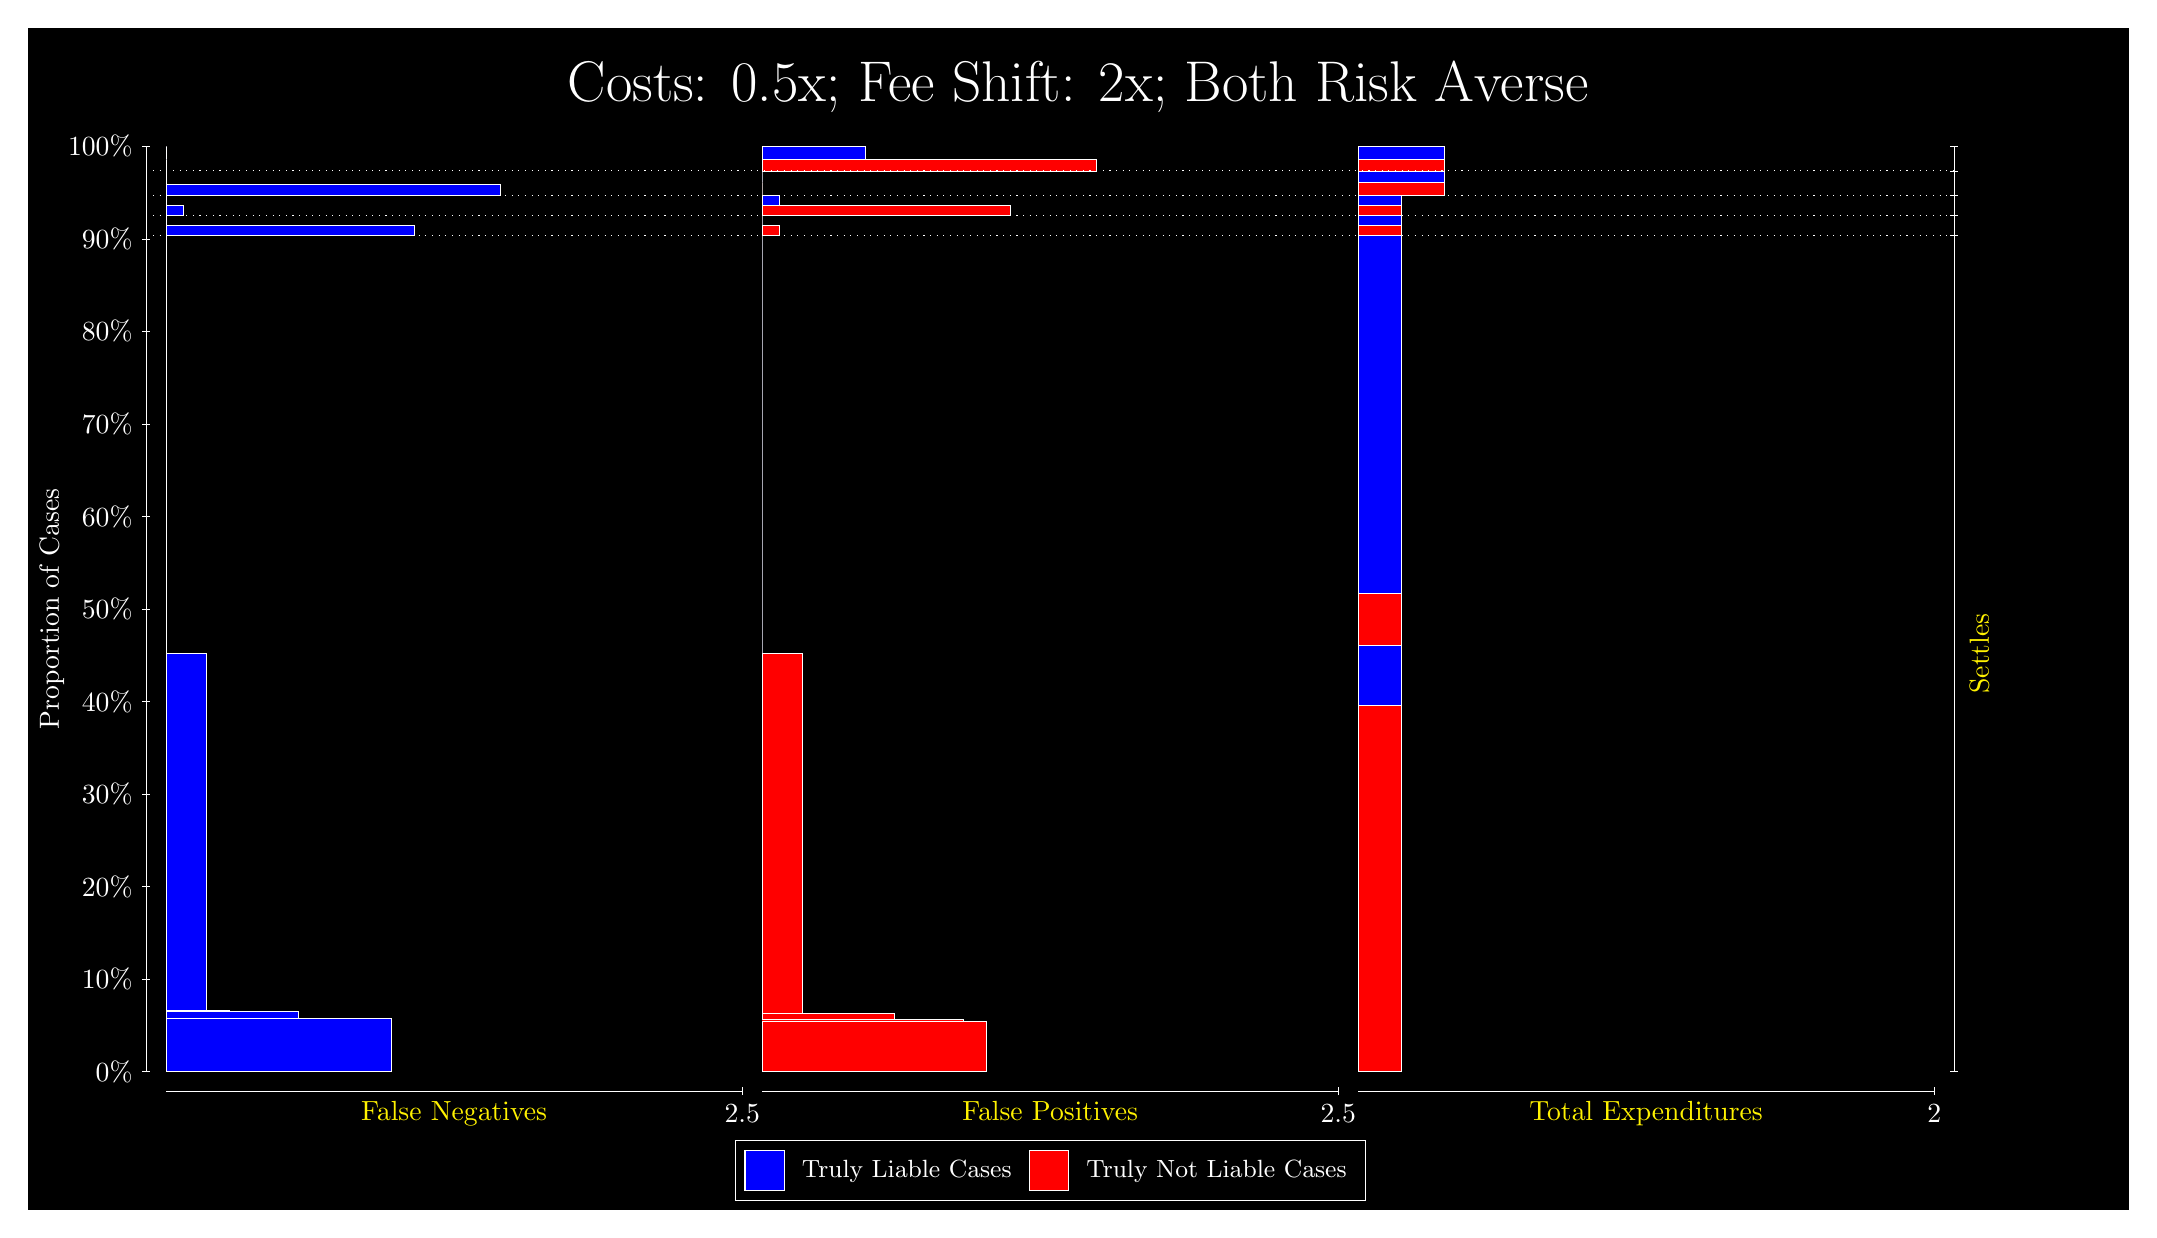
\begin{tikzpicture}
\draw[fill=black] (0,0) rectangle (26.667,15);
\draw[text=white] (0,13.5) rectangle (26.667,15) node[midway] {\huge Costs: 0.5x; Fee Shift: 2x; Both Risk Averse};
\draw[white, very thin] (1.5,1.75) -- (1.5,13.5);
\node[rotate=90, text=white, anchor=center] at (0.3, 7.625) {Proportion of Cases};
\draw[white, very thin] (1.45,1.75) -- (1.55,1.75);
\node[text=white, anchor=east] at (1.45, 1.75) {0\%};
\draw[white, very thin] (1.45,2.925) -- (1.55,2.925);
\node[text=white, anchor=east] at (1.45, 2.925) {10\%};
\draw[white, very thin] (1.45,4.1) -- (1.55,4.1);
\node[text=white, anchor=east] at (1.45, 4.1) {20\%};
\draw[white, very thin] (1.45,5.275) -- (1.55,5.275);
\node[text=white, anchor=east] at (1.45, 5.275) {30\%};
\draw[white, very thin] (1.45,6.45) -- (1.55,6.45);
\node[text=white, anchor=east] at (1.45, 6.45) {40\%};
\draw[white, very thin] (1.45,7.625) -- (1.55,7.625);
\node[text=white, anchor=east] at (1.45, 7.625) {50\%};
\draw[white, very thin] (1.45,8.8) -- (1.55,8.8);
\node[text=white, anchor=east] at (1.45, 8.8) {60\%};
\draw[white, very thin] (1.45,9.975) -- (1.55,9.975);
\node[text=white, anchor=east] at (1.45, 9.975) {70\%};
\draw[white, very thin] (1.45,11.15) -- (1.55,11.15);
\node[text=white, anchor=east] at (1.45, 11.15) {80\%};
\draw[white, very thin] (1.45,12.325) -- (1.55,12.325);
\node[text=white, anchor=east] at (1.45, 12.325) {90\%};
\draw[white, very thin] (1.45,13.5) -- (1.55,13.5);
\node[text=white, anchor=east] at (1.45, 13.5) {100\%};

\draw[white, very thin] (24.457,1.75) -- (24.457,13.5);
\draw[white, very thin] (24.407,1.75) -- (24.507,1.75);
\node[anchor=west] at (24.407, 1.75) {};
\draw[white, very thin] (24.407,12.37) -- (24.507,12.37);
\node[anchor=west] at (24.407, 12.37) {};
\draw[white, very thin] (24.407,12.625) -- (24.507,12.625);
\node[anchor=west] at (24.407, 12.625) {};
\draw[white, very thin] (24.407,12.877) -- (24.507,12.877);
\node[anchor=west] at (24.407, 12.877) {};
\draw[white, very thin] (24.407,13.188) -- (24.507,13.188);
\node[anchor=west] at (24.407, 13.188) {};
\draw[white, very thin] (24.407,13.5) -- (24.507,13.5);
\node[anchor=west] at (24.407, 13.5) {};

\draw[white, very thin, fill=blue] (1.75,1.75) rectangle (4.6044,2.4267);
\draw[white, very thin, fill=blue] (1.75,2.4267) rectangle (3.7261,2.4292);
\draw[white, very thin, fill=blue] (1.75,2.4292) rectangle (3.4333,2.5126);
\draw[white, very thin, fill=blue] (1.75,2.5126) rectangle (2.8478,2.5136);
\draw[white, very thin, fill=blue] (1.75,2.5136) rectangle (2.5551,2.5324);
\draw[white, very thin, fill=blue] (1.75,2.5324) rectangle (2.2623,7.0598);
\draw[white, very thin, fill=red] (1.75,7.0598) rectangle (1.75,12.37);
\draw[white, very thin, fill=blue] (1.75,12.37) rectangle (4.8971,12.494);
\draw[white, very thin, fill=red] (1.75,12.494) rectangle (1.75,12.625);
\draw[white, very thin, fill=blue] (1.75,12.625) rectangle (1.9696,12.755);
\draw[white, very thin, fill=red] (1.75,12.755) rectangle (1.75,12.877);
\draw[white, very thin, fill=blue] (1.75,12.877) rectangle (5.9949,13.024);
\draw[white, very thin, fill=red] (1.75,13.024) rectangle (1.75,13.188);
\draw[white, very thin, fill=red] (1.75,13.188) rectangle (1.75,13.335);
\draw[white, very thin, fill=blue] (1.75,13.335) rectangle (1.75,13.5);
\draw[white, very thin, fill=red] (9.3189,1.75) rectangle (12.173,2.3919);
\draw[white, very thin, fill=red] (9.3189,2.3919) rectangle (11.88,2.4086);
\draw[white, very thin, fill=red] (9.3189,2.4086) rectangle (11.588,2.4096);
\draw[white, very thin, fill=red] (9.3189,2.4096) rectangle (11.002,2.4924);
\draw[white, very thin, fill=red] (9.3189,2.4924) rectangle (10.709,2.4952);
\draw[white, very thin, fill=red] (9.3189,2.4952) rectangle (9.8312,7.0605);
\draw[white, very thin, fill=blue] (9.3189,7.0605) rectangle (9.3189,12.37);
\draw[white, very thin, fill=red] (9.3189,12.37) rectangle (9.5384,12.501);
\draw[white, very thin, fill=blue] (9.3189,12.501) rectangle (9.3189,12.625);
\draw[white, very thin, fill=red] (9.3189,12.625) rectangle (12.466,12.748);
\draw[white, very thin, fill=blue] (9.3189,12.748) rectangle (9.5384,12.877);
\draw[white, very thin, fill=red] (9.3189,12.877) rectangle (9.3189,13.042);
\draw[white, very thin, fill=blue] (9.3189,13.042) rectangle (9.3189,13.188);
\draw[white, very thin, fill=red] (9.3189,13.188) rectangle (13.564,13.335);
\draw[white, very thin, fill=blue] (9.3189,13.335) rectangle (10.636,13.5);
\draw[white, very thin, fill=red] (16.888,1.75) rectangle (17.437,1.7528);
\draw[white, very thin, fill=blue] (16.888,1.7528) rectangle (17.437,1.7553);
\draw[white, very thin, fill=red] (16.888,1.7553) rectangle (17.437,6.4034);
\draw[white, very thin, fill=blue] (16.888,6.4034) rectangle (17.437,7.1636);
\draw[white, very thin, fill=red] (16.888,7.1636) rectangle (17.437,7.8232);
\draw[white, very thin, fill=blue] (16.888,7.8232) rectangle (17.437,12.37);
\draw[white, very thin, fill=red] (16.888,12.37) rectangle (17.437,12.501);
\draw[white, very thin, fill=blue] (16.888,12.501) rectangle (17.437,12.625);
\draw[white, very thin, fill=red] (16.888,12.625) rectangle (17.437,12.748);
\draw[white, very thin, fill=blue] (16.888,12.748) rectangle (17.437,12.877);
\draw[white, very thin, fill=red] (16.888,12.877) rectangle (17.986,13.042);
\draw[white, very thin, fill=blue] (16.888,13.042) rectangle (17.986,13.188);
\draw[white, very thin, fill=red] (16.888,13.188) rectangle (17.986,13.335);
\draw[white, very thin, fill=blue] (16.888,13.335) rectangle (17.986,13.5);
\draw[white, dotted] (1.5,12.37) -- (24.457,12.37);
\draw[white, dotted] (1.5,12.625) -- (24.457,12.625);
\draw[white, dotted] (1.5,12.877) -- (24.457,12.877);
\draw[white, dotted] (1.5,13.188) -- (24.457,13.188);
\draw[white, very thin] (1.75,1.5) -- (9.0689,1.5);
\node[text=yellow, anchor=north] at (5.4094, 1.5) {False Negatives};
\draw[white, very thin] (9.0689,1.45) -- (9.0689,1.55);
\node[text=white, anchor=north] at (9.0689, 1.45) {2.5};

\draw[white, very thin] (9.3189,1.5) -- (16.638,1.5);
\node[text=yellow, anchor=north] at (12.978, 1.5) {False Positives};
\draw[white, very thin] (16.638,1.45) -- (16.638,1.55);
\node[text=white, anchor=north] at (16.638, 1.45) {2.5};

\draw[white, very thin] (16.888,1.5) -- (24.207,1.5);
\node[text=yellow, anchor=north] at (20.547, 1.5) {Total Expenditures};
\draw[white, very thin] (24.207,1.45) -- (24.207,1.55);
\node[text=white, anchor=north] at (24.207, 1.45) {2};

\node[text=yellow, centered, rotate=90] at (24.777, 7.0602) {Settles};





\draw (12.978300999999998,1.5) node[draw=none] (baseCoordinate) {};
\begin{scope}[align=center]
        \matrix[scale=0.5, draw=white, below=0.5cm of baseCoordinate, nodes={draw}, column sep=0.1cm]{
            \node[rectangle, draw, minimum width=0.5cm, minimum height=0.5cm, fill=blue] {}; &
            \node[draw=none, font=\small, text=white] (B) {Truly Liable Cases}; &
            \node[rectangle, draw, minimum width=0.5cm, minimum height=0.5cm, fill=red] {}; &
            \node[draw=none, font=\small, text=white] (B) {Truly Not Liable Cases}; \\
            };
\end{scope}

\end{tikzpicture}
\end{document}